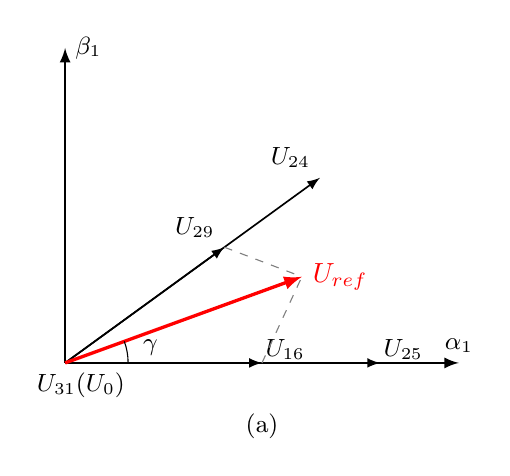
\begin{tikzpicture}[>=latex, font=\small]

    % Osy
    \draw[->, thick] (0,0) -- (5,0) node[above] {$\alpha_1$};
    \draw[->, thick] (0,0) -- (0,4) node[right] {$\beta_1$};
    \node[below] at (0.2,0) {$U_{31}(U_0)$};

    % Definice délek
    \def\Lone{2.5} 
    \def\Ltwo{4.0} 
    \def\Lref{3.2} 
    \def\angRef{20}

    % Vektory na ose alfa (U16, U25) - umístění nad šipkou
    \draw[->, semithick] (0,0) -- (\Lone,0) node[anchor=south west, inner sep=1pt] {$U_{16}$};
    \draw[->, semithick] (0,0) -- (\Ltwo,0) node[anchor=south west, inner sep=1pt] {$U_{25}$};

    % Vektory pod úhlem (U29, U24)
    \draw[->, semithick] (0,0) -- (36:\Lone) node[anchor=south east] {$U_{29}$};
    \draw[->, semithick] (0,0) -- (36:\Ltwo) node[anchor=south east] {$U_{24}$};

    % ČERVENÝ REFERENČNÍ VEKTOR Uref
    \draw[->, very thick, red] (0,0) -- (\angRef:\Lref) node[right, font=\bfseries] {$U_{ref}$};

    % Úhel gama
    \draw (0.8,0) arc (0:\angRef:0.8);
    \node at (10:1.1) {$\gamma$};

    % Konstrukční čáry
    \draw[dashed, gray] (36:\Lone) -- (\angRef:\Lref);
    \draw[dashed, gray] (\Lone,0) -- (\angRef:\Lref);

    \node at (2.5, -0.8) {(a)};

\end{tikzpicture}